\documentclass{article}\usepackage[]{graphicx}\usepackage[]{color}
%% maxwidth is the original width if it is less than linewidth
%% otherwise use linewidth (to make sure the graphics do not exceed the margin)
\makeatletter
\def\maxwidth{ %
  \ifdim\Gin@nat@width>\linewidth
    \linewidth
  \else
    \Gin@nat@width
  \fi
}
\makeatother

\definecolor{fgcolor}{rgb}{0.345, 0.345, 0.345}
\newcommand{\hlnum}[1]{\textcolor[rgb]{0.686,0.059,0.569}{#1}}%
\newcommand{\hlstr}[1]{\textcolor[rgb]{0.192,0.494,0.8}{#1}}%
\newcommand{\hlcom}[1]{\textcolor[rgb]{0.678,0.584,0.686}{\textit{#1}}}%
\newcommand{\hlopt}[1]{\textcolor[rgb]{0,0,0}{#1}}%
\newcommand{\hlstd}[1]{\textcolor[rgb]{0.345,0.345,0.345}{#1}}%
\newcommand{\hlkwa}[1]{\textcolor[rgb]{0.161,0.373,0.58}{\textbf{#1}}}%
\newcommand{\hlkwb}[1]{\textcolor[rgb]{0.69,0.353,0.396}{#1}}%
\newcommand{\hlkwc}[1]{\textcolor[rgb]{0.333,0.667,0.333}{#1}}%
\newcommand{\hlkwd}[1]{\textcolor[rgb]{0.737,0.353,0.396}{\textbf{#1}}}%
\let\hlipl\hlkwb

\usepackage{framed}
\makeatletter
\newenvironment{kframe}{%
 \def\at@end@of@kframe{}%
 \ifinner\ifhmode%
  \def\at@end@of@kframe{\end{minipage}}%
  \begin{minipage}{\columnwidth}%
 \fi\fi%
 \def\FrameCommand##1{\hskip\@totalleftmargin \hskip-\fboxsep
 \colorbox{shadecolor}{##1}\hskip-\fboxsep
     % There is no \\@totalrightmargin, so:
     \hskip-\linewidth \hskip-\@totalleftmargin \hskip\columnwidth}%
 \MakeFramed {\advance\hsize-\width
   \@totalleftmargin\z@ \linewidth\hsize
   \@setminipage}}%
 {\par\unskip\endMakeFramed%
 \at@end@of@kframe}
\makeatother

\definecolor{shadecolor}{rgb}{.97, .97, .97}
\definecolor{messagecolor}{rgb}{0, 0, 0}
\definecolor{warningcolor}{rgb}{1, 0, 1}
\definecolor{errorcolor}{rgb}{1, 0, 0}
\newenvironment{knitrout}{}{} % an empty environment to be redefined in TeX

\usepackage{alltt}
\usepackage{Sweave}
\usepackage{float}
\usepackage{graphicx}
\usepackage{tabularx}
\usepackage{siunitx}
\usepackage{mdframed}
\usepackage{natbib}
\bibliographystyle{..//refs/styles/besjournals.bst}
\usepackage[small]{caption}
\setkeys{Gin}{width=0.8\textwidth}
\setlength{\captionmargin}{30pt}
\setlength{\abovecaptionskip}{0pt}
\setlength{\belowcaptionskip}{10pt}
\topmargin -1.5cm        
\oddsidemargin -0.04cm   
\evensidemargin -0.04cm
\textwidth 16.59cm
\textheight 21.94cm 
%\pagestyle{empty} %comment if want page numbers
\parskip 7.2pt
\renewcommand{\baselinestretch}{1.5}
\parindent 0pt

\newmdenv[
  topline=true,
  bottomline=true,
  skipabove=\topsep,
  skipbelow=\topsep
]{siderules}

%% R Script


\IfFileExists{upquote.sty}{\usepackage{upquote}}{}
\begin{document}
\title{Rethinking False Spring Risk}
\author{Chamberlain, Wolkovich}
\date{\today}
\maketitle 

\renewcommand{\thetable}{\arabic{table}}
\renewcommand{\thefigure}{\arabic{figure}}
\renewcommand{\labelitemi}{$-$}

%%%%%%%%%%%%%%%%%%%%%%%%%%%%%%%%%%%%%%%%%%%%%%%
\begin{center}
\LARGE\textbf{Outline}
\end{center}
\section{Introduction}
Plants growing in temperate environments are at risk of being exposed to late spring freezes, which can be detrimental to growth. Individuals that leaf out before the last frost are at risk of leaf loss, damaging wood tissue, and slowed or stalled canopy development \citep{Gu2008, Hufkens2012}. Therefore, temperate deciduous tree species must have plastic phenological responses in the spring in order to optimize photosynthesis and minimize frost or drought risk \citep{Polgar2011}. These late spring freezing events are known as false springs. False spring events can result in highly adverse ecological and economic consequences \citep{Ault2013, Knudson2012}.

Climate change is expected to increase damage from false spring events around the world due to earlier spring onset and greater fluctuations in temperature \citep{Martin2010, Inouye2008, Cannell1986}. Temperate forest species around the world are initiating leaf out about 4.6 days earlier per degree Celsius \citep{Polgar2014, Wolkovich2012}. It is anticipated that there will be a decrease in false spring frequency overall but the magnitude of temperature variation is likely to increase, therefore amplifying the expected intensity of false spring events \citep{Allstadt2015, Kodra2011}. Multiple studies have documented false spring events in recent years \citep{Augspurger2013, Knudson2012, Augspurger2009, Gu2008} and some have linked this to climate change \citep{Muffler2016, Xin2016, Allstadt2015, Ault2013}. Due to these reasons, it is crucial for researchers to properly evaluate the effects of false spring events on temperate forests and agricultural crops in order to make more accurate predictions on future trends.

Different species respond differently to late spring freezing events. The level of damage sustained by plants from a false spring also varies across phenophases. Various studies have assessed the risk of damage or the intensity of particular false spring events but at this time false spring studies fail to incorporate all potential factors that could affect the level of frost damage risk. A False Spring Index (FSI) signifies the likelihood of a damage to occur from a late spring freeze. Currently, FSI evaluates day of budburst, number of growing degree days, and day of last spring freeze through a simple equation as seen below \citep{Marino2011}. 

\[ FSI = Julian Date (Last Spring Freeze) - Julian Date (Budburst) \]

If FSI is a positive number and greater than 7, then crown dieback is more likely to occur. False spring studies largely simplify the various ecological elements that could predict the level of plant damage from late spring freezing events. In contrast to these simplifications, we argue that a wealth of factors greatly impacts plants' frost spring risk such that simple indices will most likely lead to inaccurate predictions and ultimately do little to advance the field. 

In this paper we aim to highlight the complexity of factors driving a plant's false spring risk. We outline in particular how life stage of the individual \citep{Caffarra2011}, location within a forest or canopy \citep{Augspurger2013}, winter chilling hours (Flynn \& Wolkovich 2017?), proximity to water \citep{Gu2008}, level of precipitation prior to the freezing event \citep{Anderegg2013}, freeze duration/intensity, and range limits of the species \citep{Martin2010} unhinge simple metrics of false spring. The ultimate intent is to demonstrate how an integrated view of false spring that incorporates these factors would rapidly advance progress in this field.  

\section{Defining False Spring}
There are two phases involved in late spring freezing: rapid vegetative growth prior to the freeze and the post freeze setback. This combined process is known as a false spring \citep{Gu2008}. Freeze and thaw fluctuations can cause xylem embolism and decreased xylem conductivity which can result in crown dieback \citep{Gu2008}.

Warm temperatures earlier in the year (i.e. in February) do not seem to affect species, most likely because it is too soon for budburst to initiate and sufficient chilling has not yet occurred. Frost damage usually occurs when there is a warmer than average March, a freezing April, and enough growing days between the high temperatures and the last freeze date \citep{Augspurger2013}. 
FSI is considered significant if it is greater than 7 days between budburst and leafout \citep{Peterson2014}. The 7 day parameter exposes less resistant foliate phenophases to a freezing event and puts the plant at a higher risk of damage. Once budburst has initiated, buds cannot respond to cold temperatures and freezing resistance is greatly reduced \citep{Vitasse2014, Lenz2013, Taschler2004}. There is much debate over the definition of freezing temperatures, which has resulted in two types of freezes: a ``hard'' freeze at -2.2$^{\circ}$C and a ``soft'' freeze at -1.7$^{\circ}$C \citep{Augspurger2013, Kodra2011, Vavrus2006}.

Freezing damage can occur directly via intracellular ice formation or indirectly via freezing dehydration \citep{Hofmann2015, Beck2004, Pearce2001}. Dry winters typically results in new, frost-tolerant shoots due to the decreased water content and osmotic potential from the reduced number of accumulated solutes \citep{Hofmann2015, Morin2007}. Therefore, it is hypothesized that increased bud dehydration results in increased frost hardiness \citep{Hofmann2015, Kathke2011, Poirier2010, Nielsen2009, Beck2007}.

\subsection*{Determining Spring Onset}
Lizzie: ``I think `Determining Spring Onset'\, can go here but you need to develop idea first (e.g. canopy vs understory, species vs mix etc...) then results only and digest what they mean for reader.''

Before a suitable model for determining false spring risk can be established, an appropriate determination of spring onset is crucial. There are many methods that can be used to determine the first day of spring and there are also many definitions. Spring onset can be determined through observational data, PhenoCam or remote-sensing data, or through the USA National Phenology Network's (USA-NPN) Extended Spring Index values (SI-x) \citep{USA-NPN2016}. Observational data is frequently used because it permits researchers to identify exactly the phenophase they wish to observe and target specific species or individuals. PhenoCam or remote-sensing data is more applicable to canopy tree species and the USA-NPN SI-x is useful for understory species.

A graphical representation of the FSI values compared across the three methodologies can be seen in Figure 1. In 2008 and 2012, FSI is higher than the significant parameter given of 7 for the NPN data, indicating a possibly damaging false spring event. All three methodologies follow a similar trend except in 2012, when the PhenoCam data indicates a low risk for a false spring event but the other two indicate a false spring occurred. 

\begin{figure}[H]
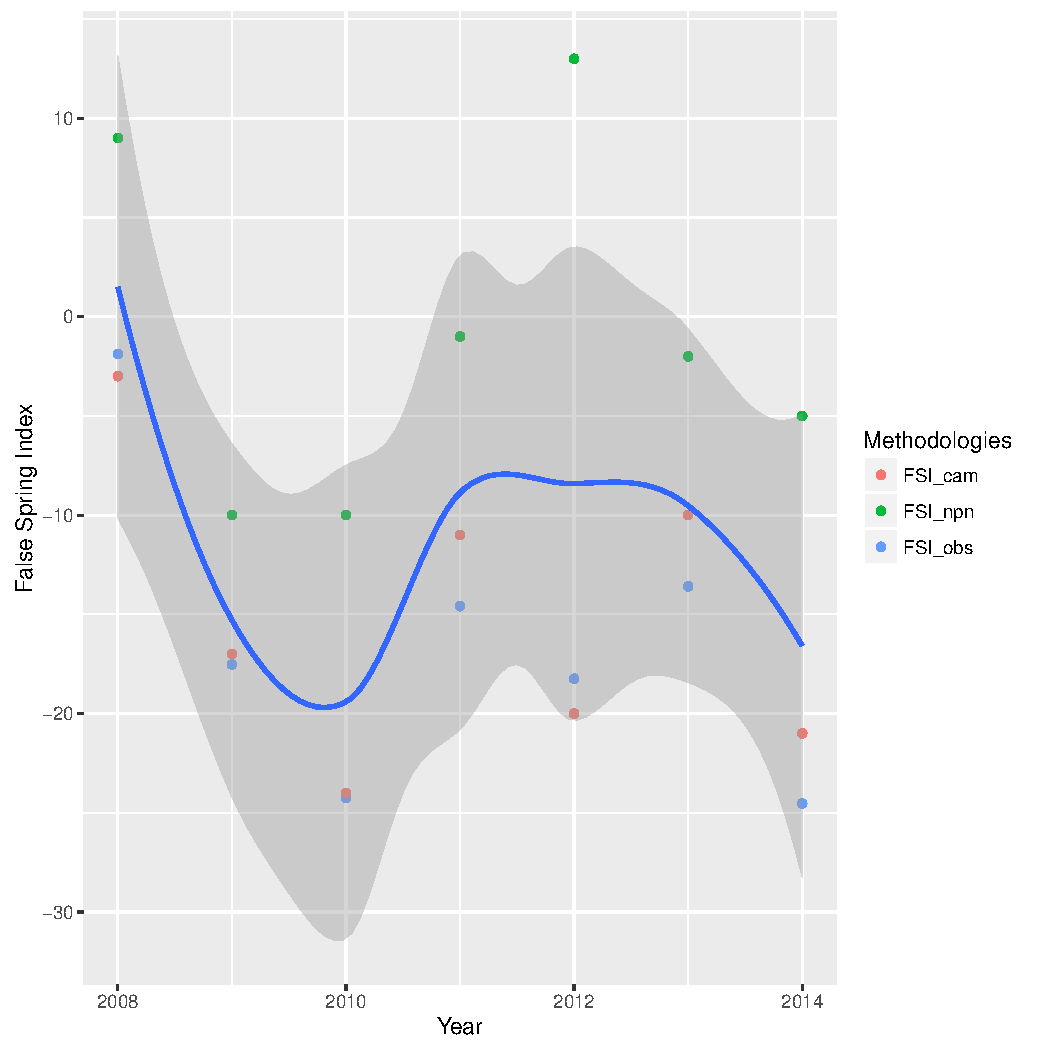
\includegraphics[width=\maxwidth]{figure/fsifig-1} \caption[A scatterplot indicating FSI values from 2008 to 2014 for each methdology used in this study]{A scatterplot indicating FSI values from 2008 to 2014 for each methdology used in this study. PhenoCam FSI values are red, Observed FSI values are blue, and USA-NPN FSI values are green.}\label{fig:fsifig}
\end{figure}



The timing of forest spring phenology progresses essentially through successional stages: understory species will initiate budburst first, then seedlings and saplings in order to exploit open canopies and early growth, whereas late successional species may start later in the season to avoid frost or drought risk \citep{Xin2016, Richardson2009}. While investigating false spring risk, forest demographics should be assessed in order to properly determine the appropriate methodology for spring onset. Pure grasslands or young forests will have early budburst dates and large stands of canopy trees will initiate budburst much later, whereas mixed forests will have a date of spring onset somewhere in between. The methodology used for determining spring onset should largely be dependent on the functional group of interest: researchers should use the USA-NPN dataset for understory species, PhenoCam or remote-sensing data for late successional species, and observational data for a wide array of plant functional types. However, through a comparative analysis assessing the three methodologies, we conclude that observational FSI values are highly comparable to the USA-NPN FSI values, rendering both justifiable methods for determining potential risk involved in late spring freezes. The PhenoCam data is also significantly related to the observational and USA-NPN data, however, it is more useful for studies primarily investigating canopy species. 

\section*{Understanding (Defining?) Vegetative Risk}
Lizzie: ``Phenophases, Species differences (maybe just set up here...), regional differences?, some of your points in Box 1 here - basically set up everything that could matter then make a case for what matters most and hit on those in next sections.''

Another highly crucial factor to consider is the rate of budburst and the length of time between budburst to full leafout, which we will refer to as the duration of vegetative risk. % repeated later in the subsection: Species Differences and Vegetative Risk, can probably take it out here

\subsection*{Phenophases}
The level of damage sustained by plants from a false spring also varies across phenophases. Generally, reproductive phases are more sensitive to false spring events than vegetative phases and developing leaves are more susceptible to damage than opening buds or expanding shoots \citep{Lenz2013,Augspurger2009}. However, trees that suffer severe vegetative growth damage from a false spring event will suffer greater long-term effects from the loss of photosynthetic tissue than trees that lose one year of reproductive growth. Spring frosts during the vegetative growth phenophases impose the greatest freezing threat to deciduous tree species \citep{Sakai1987}.

Phenophase is a greater indicator for level of risk than life stage. Individuals at a certain phenophase (i.e. between budburst and full leafout) are more likely to incur damage from a freezing event than individuals past the leafout phenophase, independent of life stage \citep{Augspurger2009,Vitasse2014}.

\subsection*{Species}
Seedlings and saplings initiate budburst before canopy closure in order to benefit from the increased light levels \citep{Augspurger2008}, therefore putting them at greater risk to false spring damage than adult trees \citep{Vitasse2014}. Younger trees are more likely to incur lastly damage to the leaf buds and vegetative growth, whereas adult trees are at risk of xylem embolism. In order for xylem embolism to occur, extreme cavitation must first occur. Extensive cavitation in the xylem would require more intensive freezing events than it would take to damage seedling and sapling leaf buds. Especially strong freezing events (i.e. >-8.6$^{\circ}$C), could result in meristemic tissue, wood parenchyma and phloem damage \citep{Lenz2013, Augspurger2011, Sakai1987}.  

However, different species respond differently to anthropogenic climate change. Most species are expected to begin leaf out earlier in the season with warming spring temperatures but some species may have the opposite response \citep{Xin2016, Cleland2006, Yu2010}.

Studies indicate that species growing at more northern latitudes tend to respond greater to photoperiod than species growing further south \citep{Caffarra2011, Viheraaarnio2006, Partanen2004}. Similarly, late successional species exhibit greater photoperiod sensitivities than pioneer species \citep{Basler2012} and they also require more chilling in the winter and greater forcing temperatures in the spring \citep{Laube2013}. 

\section*{Species Differences and Vegetative Risk}
Lizzie: ``You have so much great stuff here but need to develop WHY and HOW species would differ. You touch on this once in paper but need to develop more. This section should start with building a case for why species would differ then go into data.''

Plants are most susceptible to frost damage between budburst and leafout \citep{Lenz2016, Vitasse2014, Augspurger2009}. The rate of budburst and the length of time between budburst and leafout is a crucial indicator for predicting level of damage from a false spring event. We will refer to the timing of these collective phenophases (i.e. budburst to leafout) as the duration of vegetative risk. The duration of vegetative risk generally is extended if a freezing event occurs during the phenophases between budburst and leaf expansion and species with short durations of vegetative risk often sustain higher levels of damage. Therefore, if the duration of vegetative risk is longer, then the buds and leaves will be heartier against frosts, however this still has yet to be tested thoroughly \citep{Augspurger2009}. Frost tolerance, however, steadily decreases after budburst begins until the leaf is fully unfolded, with leafout being the most susceptible to frost damage \citep{Lenz2016}. It is therefore crucial that more studies investigate the relationship between false spring events and duration of vegetative risk. 

It is anticipated that these more opportunistic individuals that initiate budburst earlier in the spring with anthropogenic climate change would attempt to limit freezing risk by decreasing their duration of vegetative risk and progress to full leaf expansion faster than larger or more northern species. We assess this interaction using three datasets: from a citizen science program, a growth chamber chilling experiment, and long-term observational data. 

\subsection*{Treespotters Data}
We analyzed a dataset from a USA-NPN citizen science program, the Arnold Arboretum Tree Spotters %Should I mention here that it is our program or no? Also, not exactly sure how to cite it...
, to discern the relationship between duration of vegetative risk and initial budburst date. Figure 2 shows the duration of vegetative risk for 11 different species observed at the Arnold Arboretum in 2016. \textit{Quercus alba} and \textit{Betula nigra} had the longest durations of vegetative risk, most likely due to the fact that one is late successional species and the other is northern species respectively. Overall, there is no significant relationship between duration of vegetative risk and day of budburst. This could be due to the fact that there are various functional groups involved in this study, that it is just over the course of one year, that it is in an arboretum, and that it is a citizen science project. Further investigations should be made to gain a better understanding of observational studies for this interaction. 


%Appears to be a relationship between successional status and duration of vegetative risk. Check out if there's a statistical relationship...

\begin{figure}[H]
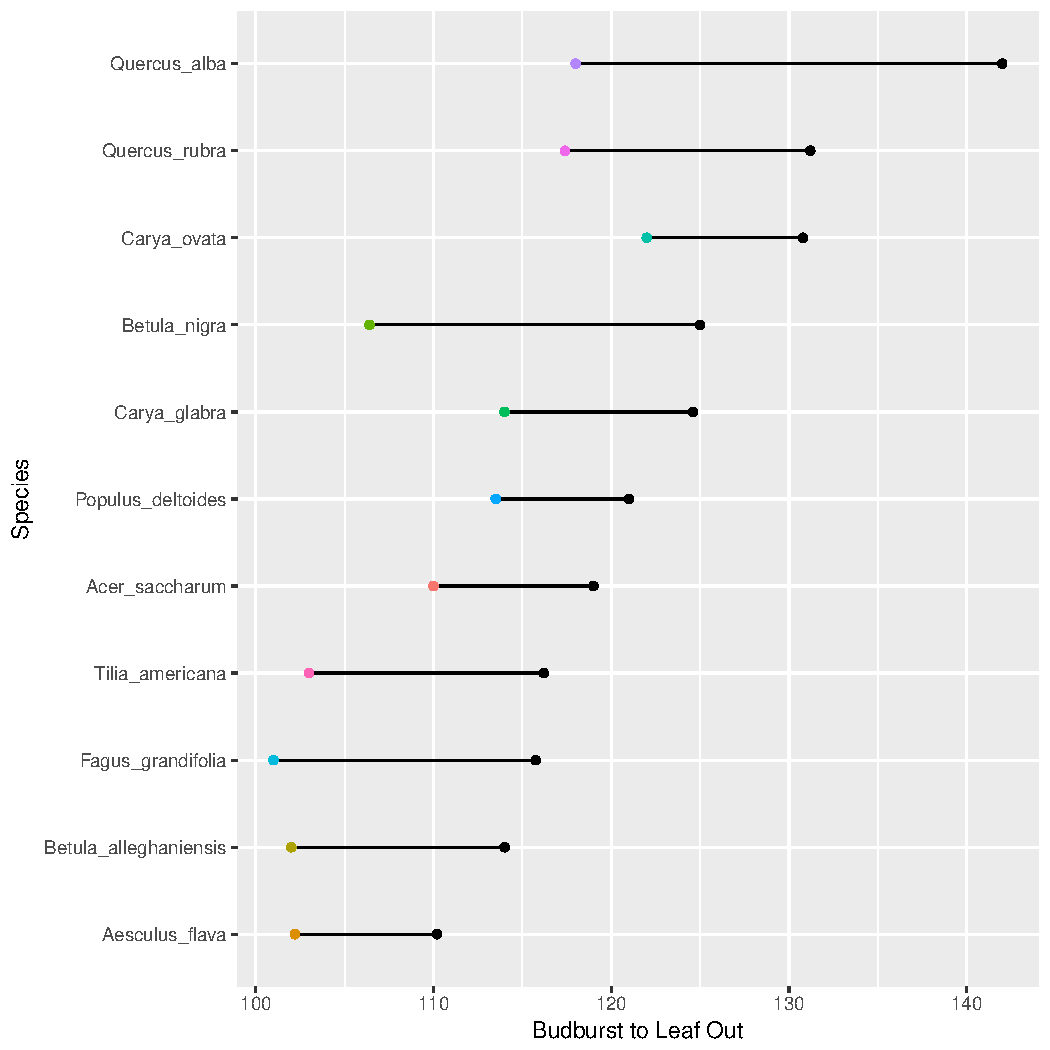
\includegraphics[width=\maxwidth]{figure/treespotters-1} \caption[A timeline plot indicating the duration of vegetative risk for each species studied at the Arnold Arboretum in 2016]{A timeline plot indicating the duration of vegetative risk for each species studied at the Arnold Arboretum in 2016.}\label{fig:treespotters}
\end{figure}



\subsection*{Dan's Data}
It is possible, that with anthropogenic climate change progressing, leaf out timing may be delayed. As winter seasons begin to warm and chilling requirements are not met, more warming in the spring must first occur for budburst to begin \citep{Chuine2010, Polgar2014, Fu2012, Morin2009, McCreary1990}. In a chilling experiment , there were various experimental chilling, photoperiod, and forcing treatments (Flynn \& Wolkovich, ?). In Figure 2, five species were assessed across five different treatments. C is a forcing temperature of 15$^{\circ}$C during the day and 5$^{\circ}$C at night, W is a forcing temperature of 20$^{\circ}$C during the day and 10$^{\circ}$C at night, S is a short day with 8 hours of daylight, L is a long day with 12 hours of daylight, 0 is no additional winter chilling, 1 is 33 days of additional winter chilling at 4$^{\circ}$C, and 2 is 33 days of additional winter chilling at 1.5$^{\circ}$C. QUERUB is \textit{Quercus rubra}, ACERUB is \textit{Acer rubrum}, POPGRA is \textit{Populus grandidentata}, ILEMUC is \textit{Ilex mucronata}, BETPAP is \textit{Betula papyrifera}. Anova results indicate that chilling has a similar effect on budburst and leafout but photoperiod and forcing temperatures have varying effects on the two phenophases resulting in changes in duration of vegetative risk. This should be analyzed further in future studies. 

\begin{kframe}


{\ttfamily\noindent\bfseries\color{errorcolor}{\#\# Error in file(con, "{}r"{}): cannot open the connection}}\end{kframe}\begin{figure}[H]
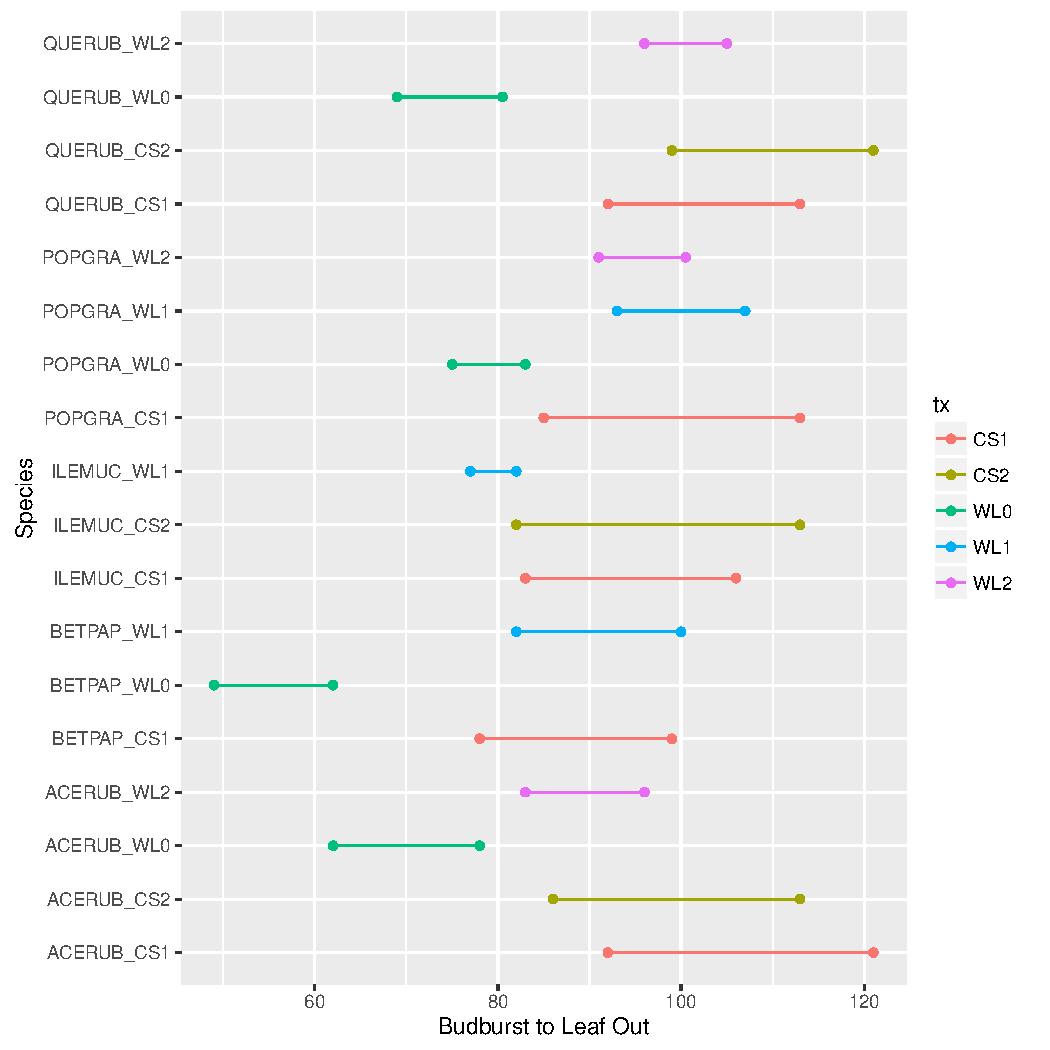
\includegraphics[width=\maxwidth]{figure/chilling-1} \caption[A timeline plot indicating the duration of vegetative risk for each species from experimental chilling study]{A timeline plot indicating the duration of vegetative risk for each species from experimental chilling study.}\label{fig:chilling}
\end{figure}



As seen in Table 5, the warmer forcing temperatures (20$^{\circ}$C during the day and 5$^{\circ}$ at night) had the greatest affect on duration of vegetative risk. High forcing temperatures greatly reduced the length of time it took between budburst and leaf out for all species. 

\begin{kframe}


{\ttfamily\noindent\color{warningcolor}{\#\# Warning in file(con, "{}r"{}): cannot open file '..//scripts/dans.timeline.R': No such file or directory}}

{\ttfamily\noindent\bfseries\color{errorcolor}{\#\# Error in file(con, "{}r"{}): cannot open the connection}}\end{kframe}
% Table created by stargazer v.5.2 by Marek Hlavac, Harvard University. E-mail: hlavac at fas.harvard.edu
% Date and time: Wed, May 31, 2017 - 08:36:18
\begin{table}[!htbp] \centering 
  \caption{The results from a linear regression model analyzing the relationship between duration of vegetation risk and intial budburst across five treatments} 
  \label{} 
\begin{tabular}{@{\extracolsep{5pt}}lc} 
\\[-1.8ex]\hline 
\hline \\[-1.8ex] 
 & \multicolumn{1}{c}{\textit{Dependent variable:}} \\ 
\cline{2-2} 
\\[-1.8ex] & Risk \\ 
\hline \\[-1.8ex] 
 Budburst & $-$0.094 \\ 
  & (0.144) \\ 
  txCS2 & 2.550 \\ 
  & (3.179) \\ 
  txWL0 & $-$14.376$^{***}$ \\ 
  & (4.315) \\ 
  txWL1 & $-$12.256$^{***}$ \\ 
  & (3.163) \\ 
  txWL2 & $-$13.522$^{***}$ \\ 
  & (3.202) \\ 
  Constant & 32.522$^{**}$ \\ 
  & (12.521) \\ 
 \hline \\[-1.8ex] 
Observations & 18 \\ 
R$^{2}$ & 0.790 \\ 
Adjusted R$^{2}$ & 0.703 \\ 
Residual Std. Error & 4.313 (df = 12) \\ 
F Statistic & 9.031$^{***}$ (df = 5; 12) \\ 
\hline 
\hline \\[-1.8ex] 
\textit{Note:}  & \multicolumn{1}{r}{$^{*}$p$<$0.1; $^{**}$p$<$0.05; $^{***}$p$<$0.01} \\ 
\end{tabular} 
\end{table} 


\subsection*{Harvard Forest Data}
The final dataset for measuring duration of vegetative risk against initial day of budburst is from John O'Keefe's observational data that was also used in the \textit{Determining Spring Onset} section. For this portion of the study, we assessed two years of data: one year that had an unusually early spring onset (2010) and another year that had an unusually late spring (2014). QUAL is \textit{Quercus alba}, FRAM is \textit{Fraxinus americana}, BEAL is \textit{Betula alleghaniensis}, ACRU is \textit{Acer rubrum}, FAGR is \textit{Fagus grandifolia}, ACPE is \textit{Acer pensylvanicum}, QURU is \textit{Quercus rubra}, and HAVI is \textit{Hamamelis virginiana}. As is evident in Figure 4, the duration of vegetative risk is slightly longer in 2010 which was when spring onset was unusually early, which could be from lower forcing temperatures. Given the paucity of information and the disparate results across the three studies assessing duration of vegetative risk, more research should be done in order to better understand this relationship. 


\begin{figure}[H]
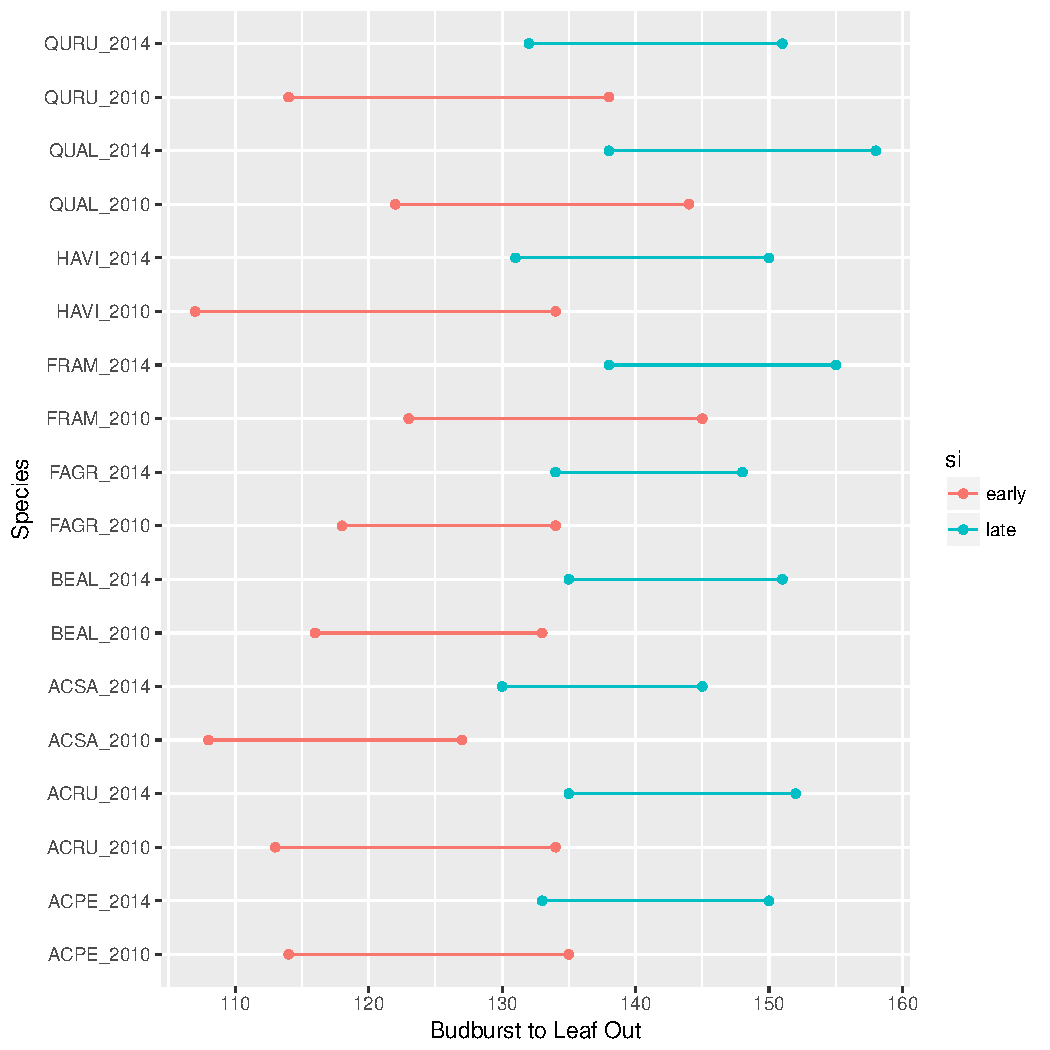
\includegraphics[width=\maxwidth]{figure/forest-1} \caption[A timeline plot indicating the duration of vegetative risk for each species from collected from Harvard Forest]{A timeline plot indicating the duration of vegetative risk for each species from collected from Harvard Forest.}\label{fig:forest}
\end{figure}




\section*{Regional Differences in Vegetative Risk?}
Lizzie: ``Again need to build up for readers why regions might differ and how (basically get your readers to come up with your hypothesis before you spell it out) then 1) analyze lit for regional differences b) latitude analysis. And maybe a few other points you make here fit.''

The reason more northern species respond more to photoperiodic cues is generally thought to be because it is a safer strategy to limit risk of exposure to false spring events \citep{Polgar2011}. However, this trend could also imply that the risk of late spring freezing events is lower at higher latitudes and species can more or less ignore temperature cues. If day length is long enough for spring budburst to initiate, but temperatures are still low, the risk of frost damage is generally lower overall at higher latitudes. This relationship must be further tested to better understand exactly what latitudes are at risk. However, researchers must bear in mind that this region of risk could shift as anthropogenic climate change progresses. 

%OR even more simply, temperature and photoperiod more closely coincide at higher latitudes.

%OR even MORE simply, false springs are only a real concern at certain latitudes.

\begin{figure} [H]
\begin{center}
\caption{Number of False Springs across two latitudinal gradients from 1986-2016: the plot on the left is the North American transect and the plot on the right is the European transect. More red dots have fewer false springs, whereas blue dots have more false springs. The size of the dot corresponds to frequency of false springs over the 30 year time frame. False spring events were calculated by using just meteorological data. Growing degree days were considered anything over 10$^{\circ}$C. A false spring event would not count if it was before early to mid March and if there were not at least 40 growing degree days before the daily mean temperature went below 0$^{\circ}$C.}
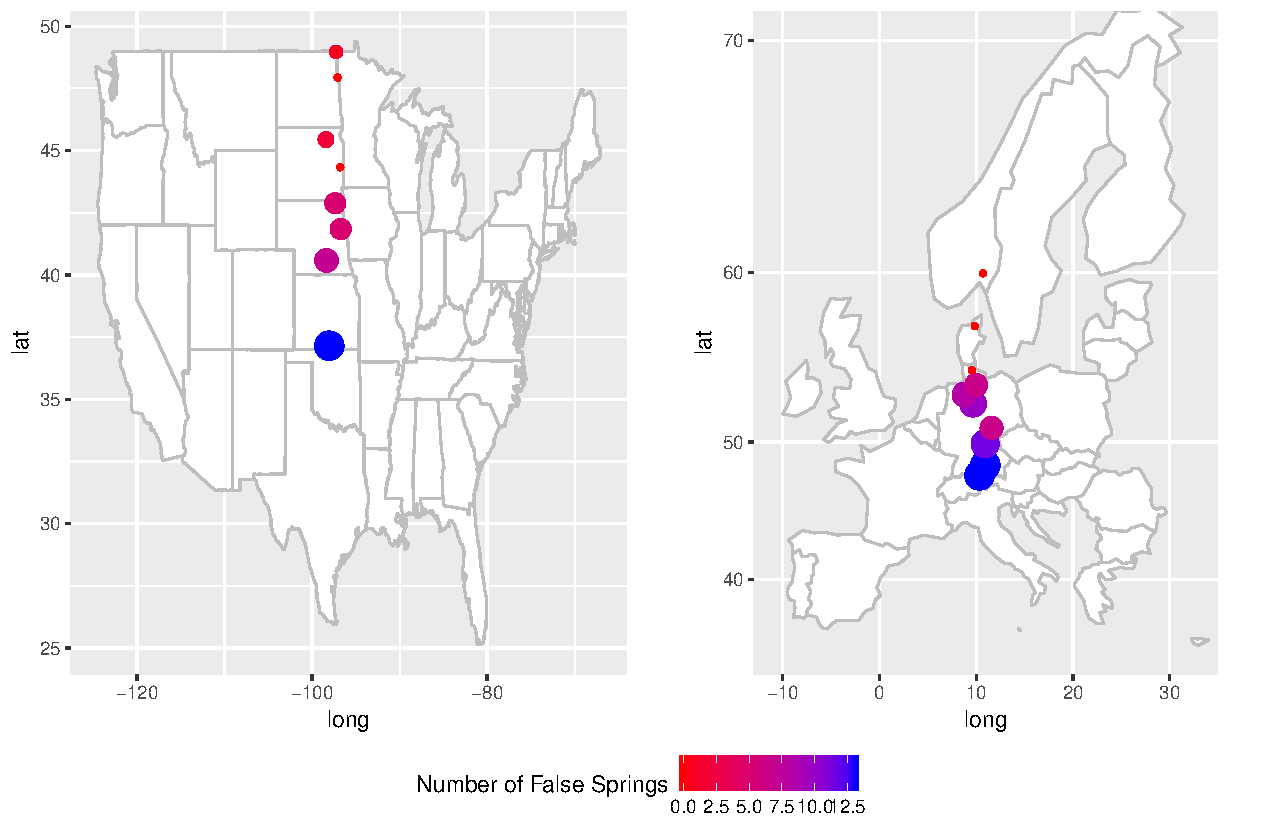
\includegraphics[width=18cm, height=10cm]{..//figure/lat.pdf} %Lat.Map.R save as 8.5x5.5
\end{center}
\end{figure}

Table 4 shows the results from the linear regression models performed for both transects. Latitude (1) represents the European transect and Latitude (2) is the American transect. 

\begin{kframe}


{\ttfamily\noindent\color{warningcolor}{\#\# Warning in file(con, "{}r"{}): cannot open file '..//scripts/Weather\_Latitude.R': No such file or directory}}

{\ttfamily\noindent\bfseries\color{errorcolor}{\#\# Error in file(con, "{}r"{}): cannot open the connection}}\end{kframe}
% Table created by stargazer v.5.2 by Marek Hlavac, Harvard University. E-mail: hlavac at fas.harvard.edu
% Date and time: Wed, May 31, 2017 - 08:36:18
\begin{table}[!htbp] \centering 
  \caption{The results from a linear regression model analyzing the relationship between latitude and frequency of false springs} 
  \label{} 
\begin{tabular}{@{\extracolsep{5pt}}lcc} 
\\[-1.8ex]\hline 
\hline \\[-1.8ex] 
 & \multicolumn{2}{c}{\textit{Dependent variable:}} \\ 
\cline{2-3} 
\\[-1.8ex] & \multicolumn{2}{c}{Latitude} \\ 
\\[-1.8ex] & (1) & (2)\\ 
\hline \\[-1.8ex] 
 False.Springs & $-$1.064$^{***}$ & $-$0.801$^{***}$ \\ 
  & (0.180) & (0.148) \\ 
  Constant & 57.235$^{***}$ & 46.946$^{***}$ \\ 
  & (0.936) & (0.865) \\ 
 \hline \\[-1.8ex] 
Observations & 10 & 8 \\ 
R$^{2}$ & 0.813 & 0.830 \\ 
Adjusted R$^{2}$ & 0.790 & 0.801 \\ 
Residual Std. Error & 1.743 (df = 8) & 1.732 (df = 6) \\ 
F Statistic & 34.885$^{***}$ (df = 1; 8) & 29.251$^{***}$ (df = 1; 6) \\ 
\hline 
\hline \\[-1.8ex] 
\textit{Note:}  & \multicolumn{2}{r}{$^{*}$p$<$0.1; $^{**}$p$<$0.05; $^{***}$p$<$0.01} \\ 
\end{tabular} 
\end{table} 


As seen in the above tables, as latitude increases the frequency of false spring events decreases. These results may indicate why species with a more northern range may have greater photoperiod sensitivities \citep{Caffarra2011} because the level of risk associated with a frost may in fact decrease. These findings demonstrate that further research is needed but they could ultimately indicate that certain latitudes should be prioritized for future false spring studies. 

\section*{Conclusion}
With anthropogenic climate change, false spring risk is higher and the level of damage expected is also greater. Furthermore, habitat fragmentation is increasing. Understanding the impact of false springs on forest communities, especially along forest edges, would be invaluable. The climatic implications suggest spring forcing temperatures will increase, thus resulting in potentially earlier date of budburst and increased risk for frost or drought damage. However, as is evident from the latitudinal gradients, risk may be greater at certain latitudes. By simply using climate data for this analysis, it shows that the level of risk is simply a regional effect rather than species or functional group specific. The interaction of species and functional group with latitude should be investigated. Calculating spring onset as accurately as possible is essential in order to determine the intensity of a false spring event. Therefore, integrating functional group within a community should be evaluated prior to choosing a method for determining spring onset. Finally, the duration of vegetative risk must be assessed further. The three study types suggest various results with the clearest indication being that greater forcing temperatures in the spring will result in shorter and earlier durations of vegetative risk. Future studies should look at the relationship between phenological plasticity and duration of vegetative risk as well as level of damage in relation to duration of vegetative risk. Box 1 is a list of all the key indicators necessary at this time to properly evaluate false spring risk and damage. These indicators should first be tested for significance and then integrated into a model for agricultural and ecological projections. 

\captionsetup[table]{textformat=empty,labelformat=empty}
\captionof{table}{Key Indicators for Modeling False Spring Risk and Damage}
\begin{siderules}
\textbf {Box 1: Key Indicators for Modeling False Spring Risk and Damage}\\
In order to properly evaluate the expected level of damage sustained from a false spring event
key indicators should be included in the model.
\renewcommand{\theenumi}{\Roman{enumi}}
\renewcommand{\theenumii}{\roman{enumii}}
\begin{enumerate}
  \item Life Stage of the Individual(s) \citep{Caffarra2011}
  \begin{enumerate}
    \item Seedlings and saplings will begin budburst earlier than adults
    \item The duration of vegetative risk may vary between life stages
    \item Long-term effects may vary
  \end{enumerate}
  \item Location Within a Forest \citep{Augspurger2013}
  \begin{enumerate}
    \item Individuals along the forest edge are more likely to experience a false spring
    \item Level of damage is likely to be higher at forest edges
  \end{enumerate}
  \item Amount of Winter Chilling (Flynn \& Wolkovich, 2017?)
  \begin{enumerate}
    \item Will affect the timing of budburst in the spring
    \item Will affect the duration of vegetative risk
  \end{enumerate}
  \item Proximity to Water %\citep{Gu2008}
  \begin{enumerate}
    \item Large bodies of water are expected to act as a buffer to spring freezes
  \end{enumerate}
  \item Precipitation Prior to Budburst \citep{Anderegg2013}
  \begin{enumerate}
    \item Will a drought increase cavitation and heighten damage from a false spring?
    \item Or will a drought decrease the risk of damage due to a lower chance of intracellular frost damage?
  \end{enumerate}
  \item Freeze Duration and Intensity
  \begin{enumerate}
    \item How should we define freezing temperatures?
    \item At what point is a freezing event severely damaging and xylem embolism occurs?
    \item How long must a false spring be to cause xylem embolism?
  \end{enumerate}
  \item Range of the Species
  \begin{enumerate}
    \item Species that have a more northern range may be more photoperiod than temperature sensitive 
  \end{enumerate}
\end{enumerate}
\end{siderules}


\newpage
\bibliography{..//refs/SpringFreeze.bib}
\end{document}

\section*{Supplemental Information}
\subsection*{Determining Spring Onset}
In order to test the best technique for calculating spring onset (or budburst), we gathered data using three different methodologies. The first method for collecting budburst was from observational data recorded for 33 tree species by Dr. John O'Keefe at Harvard Forest from 1990 to 2014 \citep{OKeefe2014}. 
Dr. O'Keefe defines budburst as 50\% green tip emergence. We subsetted this dataset to include only the tree species that were most consistently observed, which ended up being eight species.

The second dataset was from PhenoCam data, which are field cameras placed in the Harvard Forest canopy that take real-time images of plant growth and are programmed to record initial green up. The final set was collected through the USA National Phenology Network (USA-NPN), using their Data Visualization tool to gather Extended Spring Index values (SI-x) by accessing the "Spring Indices, Historic Annual" gridded layer and looking specifically at "First Leaf - Spring Onset" \citep{SI-x2016}. The SI-x value uses the time of leaf out using historical dates of budburst from honeysuckle and lilac clones around the U.S. and combines that information with daily recordings from local weather stations \citep{USA-NPN2016, Ault2015, Ault2015a, Schwartz2013, Schwartz1997}. 
Through assessing past years' weather and budburst, scientists are able to determine general weather trends that subsequently lead to leaf out. Based on these trends, SI-x values can be calculated from daily weather data \citep{USA-NPN2016}.
\par
The date of last spring freeze was gathered from the Fisher Meteorological Station which was downloaded from the Harvard Forest web page (data available online\footnote{http://harvardforest.fas.harvard.edu/meteorological-hydrological-stations}). The $T_{min}$ values were used and the last spring freeze was determined from the latest spring date that the temperature reached -1.7$^{\circ}$C or below. 
\par
PhenoCam data is not available for Harvard Forest until 2008 and observation data is only recorded through 2014, so this evaluation assesses FSI values from 2008 through 2014.
The FSI values were calculated for each methodology using the formula based on the study performed by Marino et al. (2011). Table 2 shows that the Observed and PhenoCam FSI values are all negative from 2008 through 2014, except for 2012 when the observational data indicates a false spring event. The FSI values from the USA-NPN are typically much higher in comparison to the other two methods.  
\par
A Pearson Correlation was used to determine the strength of association between the three methods used in the study. As indicated in Table 1, the FSI values from the observed data and the SI-x NPN data are strongly correlated (r=0.9395), whereas the FSI values calculated using the PhenoCam data is not as strongly correlated to either the observed FSI values (r=0.4680) or the NPN FSI values (r=0.4242). Although, according to the Pearson correlation, all methods were considered to be significantly related. 

\begin{table}[ht]
\centering
\caption{Pearson Correlation Coefficients indicating the strength of association between the FSI values calculated across all three methodologies.} 
\begin{tabular}{rrrrr}
  \hline
 & year & npn & okeefe & phenocam \\ 
  \hline
year & 1.00 & -0.03 & -0.20 & -0.37 \\ 
  npn & -0.03 & 1.00 & 0.94 & 0.42 \\ 
  okeefe & -0.20 & 0.94 & 1.00 & 0.47 \\ 
  phenocam & -0.37 & 0.42 & 0.47 & 1.00 \\ 
   \hline
\end{tabular}
\end{table}


\subsection*{Species Differences and Vegetative Risk}


Table 1 shows the results from the European transect investigated. False spring occurrence ranged from 0 to 8 and increased as latitude decreased. 

\begin{center}
\captionof{table}{Number of False Springs along a Latitudinal Gradient in Western Europe} \label{tab:title} 
\begin{tabular}{c c c c c}
\hline
Station & Elevation & Latitude & Longitude & False Springs \\
\hline
Kempten, Germany & 705m & 47.724 & 10.336 & 8 \\
Augsburg, Germany & 461m & 48.426 & 10.943 & 8 \\
Bamberg, Germany & 210m & 49.875 & 10.921 & 7 \\
Jena, Germany & 155m & 50.927 & 11.584 & 4 \\
Hannover, Germany & 55.0m & 52.466 & 9.679 & 6 \\
Bremen, Germany & 4.00m & 53.046 & 8.799 & 5 \\
Hamburg, Germany & 11.0m & 53.635 & 9.99 & 4 \\
Schleswig, Germany & 43.0m & 54.529 & 9.549 & 0 \\
Flyvestation, Denmark & 3.00m & 57.093 & 9.849 & 0 \\
Oslo, Norway & 94.0m & 59.943 & 10.721 & 0 \\
\hline
\end{tabular}
\end{center}

\subsection*{Regional Differences in Vegetative Risk}
Based on this information, we analyzed two latitudinal gradients by downloading Daily Summary climate datasets from the NOAA Climate Data Online tool. We assessed 8-10 different degree latitude lines for each transect in order to measure frequency of false spring events \citep{Menne2012, Menne2012b}. False springs were tallied by first calculating the number of Growing Degree Days (GDD) with a base 10$^{\circ}$C temperature \citep{Nugent2005}.

If there were 40 GDDs before a hard freeze occurred in the spring (-2.2$^{\circ}$C), then it was determined that a false spring could have occurred in that year. Since we did not incorporate actual budburst or spring onset information, it is unclear whether these events were actually damaging. In order to simply address the climate question, we used these parameters to have a better understanding of the potential climate effects of latitude. 

Each location includes 30 years of climate data and each transect fell within 3 degrees longitude. Locations that were over 1,000m above sea level were excluded. 

Table 2 shows the results from the American transect. False spring occurrence ranged from 0 to 13 and also exhibited an inverse relationship with latitude. 

\begin{center}
\captionof{table}{Number of False Springs along a Latitudinal Gradient in North America} \label{tab:title2} 
\begin{tabular}{c c c c c}
\hline
Station & Elevation & Latitude & Longitude & False Springs \\
\hline
Anthony, Kansas & 415m & 37.155 & -98.028 & 13 \\
Hastings, Nebraska & 587m & 40.583 & -98.350  & 7 \\
West Point, Nebraska & 399m & 41.845 & -96.714 & 5 \\
Yankton, South Dakota & 360m & 42.883 & -97.350 & 5 \\
Brookings, South Dakota & 497m & 44.325 & -96.769 & 0 \\
Aberdeen, South Dakota & 395m & 45.443 & -98.413 & 2 \\
Grand Forks, North Dakota & 253m & 47.933 & -97.083 & 0 \\
Pembina, North Dakota & 241m & 48.971 & -97.242 & 1 \\
\hline
\end{tabular}
\end{center}
